\documentclass{beamer}
\usepackage{pgfplots}
\usetheme{Boadilla}
 
 
\title{Analizador L\'exico}
\subtitle{Proyecto 1}
\author{Ariana Berm\'udez,Ximena Bola\~nos, Dylan Rodr\'iguez}
\institute{Instituto Tecnol\'ogico de Costa Rica}
\date{\today}
\begin{document}
\begin{frame}
 \titlepage 
 \end{frame}\begin{frame}
 \frametitle{An\'alisis L\'exico}
 Se hizo un analizador l\'exico con la ayuda de la herramienta Flex, para el lenguaje C, este analizador encuentra los tokens y busca su tipo, y incrementa el contador de ese tipo para luego generar histogramas y gr\'aficos de queques. Estos gr\'aficos son mostrados en una presentaci\'on de beamer, que ser\'a tambi\'en la salida del Scanner. \end{frame}\begin{frame}
 \frametitle{FLEX}
 Herramienta utilizada para realizar \'escaneres. Este toma los valores de entrada y genera los tokens correspondientes.Seg\'un la necesidad del programador. \\ Este genera un c\'odigo fuente en C que se va a nombrar lex.yy.c en el cual se genera una funci\'on yylex() la cu\'al se encarga de analizar el c\'odigo fuente. Busca la librer\'ia –lfl después de ser compilado y se enlaza con ella, para dar como resultado un ejecutable. \\ 
 El fichero de entrada de flex tiene 3 secciones, y tiene que verse como:\\ 
 \textcolor{blue}{definiciones \\ \%\% \\ reglas \\ \%\% \\ c\'odigo de usuario} \\ 
\end{frame}
\begin{frame}
Las definiciones contienen las declaraciones de nombres, y condiciones de arranque. Un ejemplo de nuestro programa es: \newline 
\textcolor{red}{[a-zA-Z][\_a-zA-Z0-9]*   return IDENTIFIER; \newline [0-9][0-9]*    return INTEGER;} \newline 
Luego de definir estos campos se procede a explicar como funciona flex, el flex asocia las entradas, \textbf{?`pero c\'omo lo hace?}\newline 
El esc\'aner analiza poco a poco las cadenas hasta que concuerden con alg\'un patr\'on propuesto por el programador. Si se puede emparejar m\'as de una forma entonces tiene prioridad quien pueda asociar m\'as texto y si en ese caso tambi\'en son iguales entonces se elige por medio de quien est\'e antes en el fichero de entrada.\newline 
El token tendr\'a asociado el puntero a caracter global \textbf{yytext}, y la longitud en la variable global entera \textbf{yyleng}. Si no hay forma de asociarlo, se usa la regla por defecto. \newline 
\end{frame}
\begin{frame}
\frametitle{FLEX - continuaci\'on} 
\textbf{Acciones} \newline 
Todo patr\'on tiene una acci\'on asociada. Existen varias acciones, por ejemplo: si se pone \newline 
\begin{table}[]
\centering
\caption{Acciones}
\label{Acciones}
\begin{tabular}{|l|l|}
 \hline 
\%\% "texto" & Har\'a que se borren todas sus aparciones en la entrada. \\ \hline 
\{ & \begin{tabular}[c]{@{}l@{}}Tomar\'a todo eso como parte de la acci\'on hasta \\ que encuentre la llave que lo cierra, \}.\end{tabular} \\ \hline 
| & Hace que la acci\'on actual aplique tambi\'en para la siguiente. \\ \hline  
\end{tabular} 
\end{table} 
El yylex() es una funci\'on que procesa tokens desde donde lo dejaron la \'ultima vez. Directivas especiales que se pueden incluir dentro de una acci\'on\end{frame}
\begin{frame}
\frametitle{C\'odigo Analizado}
\textcolor{purple}{/*hola*/} \textcolor{magenta}{int} \textcolor{green}{i} \textcolor{blue}{=} \textcolor{red}{0} \textcolor{orange}{;} \\ 
 \textcolor{magenta}{while} \textcolor{orange}{(} \textcolor{green}{i} \colorbox{red}{.}\textcolor{blue}{!=} \textcolor{red}{10} \textcolor{orange}{)} \textcolor{orange}{\{} \\ 
 \textcolor{green}{i} \textcolor{blue}{++} \textcolor{orange}{;} \\ 
 \textcolor{orange}{\}} \\ 
 \textcolor{white}{} \end{frame}
\begin{frame}
\frametitle{Histograma}
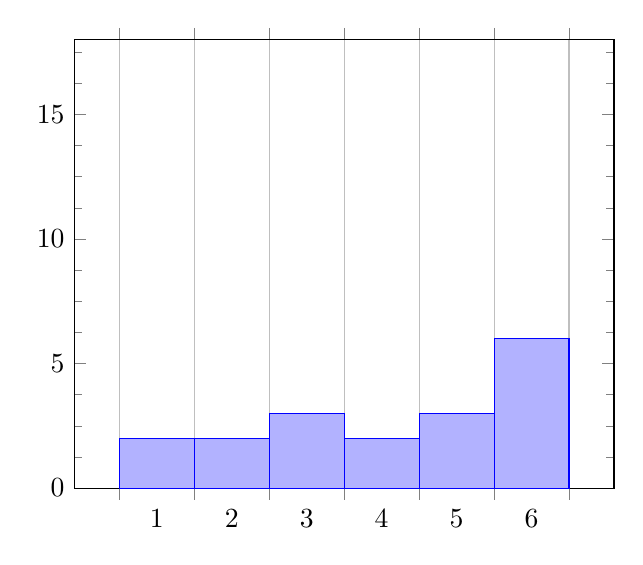
\begin{tikzpicture}
\begin{axis}[ybar interval, ymax=18, ymin=0, minor y tick num = 3]
\addplot coordinates { (1 , 2) (2 , 2) (3 , 3) (4 , 2) (5 , 3) (6 , 6)  (7, 0) }; 
\end{axis}
\end{tikzpicture}
\end{frame}
\begin{frame}
\frametitle{Histograma tipo Pastel}
\def\angle{0}
\def\radius{3}
\def\cyclelist{{"yellow","blue","red","green"}}
\newcount\cyclecount \cyclecount=-1
\newcount\ind \ind=-1
\begin{tikzpicture}[nodes = {font=\sffamily}]
\foreach \percent/\name in {
11/KEYWORD,
11/INTEGER,
16/IDENTIFIER,
11/CONSTANT,
16/OPERATOR,
33/PUNTUACTOR
 } {
\ifx\percent\empty\else
\global\advance\cyclecount by 1
\global\advance\ind by 1
\ifnum3<\cyclecount
\global\cyclecount=0
\global\ind=0
\fi
\pgfmathparse{\cyclelist[\the\ind]}
\edef\color{\pgfmathresult}
\draw[fill={\color!50},draw={\color}] (0,0) -- (\angle:\radius)
arc (\angle:\angle+\percent*3.6:\radius) -- cycle;
\node at (\angle+0.5*\percent*3.6:0.7*\radius) {\percent\,\%};
\node[pin=\angle+0.5*\percent*3.6:\name]
at (\angle+0.5*\percent*3.6:\radius) {};
\pgfmathparse{\angle+\percent*3.6}
\xdef\angle{\pgfmathresult} % and store in \angle
\fi
};
\end{tikzpicture}

\end{frame}
\end{document}
